\documentclass[a4paper,11pt]{article}

\title{A sample Sweave demo}
\author{Author name}
\date{}

\usepackage{Sweave}
\begin{document}
\Sconcordance{concordance:sweave.test1.tex:sweave.test1.Rnw:%
1 6 1 1 0 8 1 1 6 1 2 1 0 3 1 1 3 1 0 1 2 1 1 1 3 2 0 1 5 7 0 1 2 2 1 2 %
2 4 1}




\setkeys{Gin}{width=0.6\textwidth}

\maketitle


\begin{Schunk}
\begin{Sinput}
> n <- 1000
> x <- rnorm(n, mean=2)
> y <- 1.5 + 0.4*x + rnorm(n)
> df <- data.frame(x=x, y=y)
> # take a bootstrap sample
> df <- df[sample(nrow(df), nrow(df), rep=TRUE),]
> xc <- with(df, xyTable(x, y))
> df2 <- cbind.data.frame(x=xc$x, y=xc$y, n=xc$number)
> df.ell <- as.data.frame(with(df, ellipse(cor(x, y), 
+                                          scale=c(sd(x),sd(y)), 
+                                          centre=c(mean(x),mean(y)))))
> p1 <- ggplot(data=df2, aes(x=x, y=y)) + 
+   geom_point(aes(size=n), alpha=.6) + 
+   stat_smooth(data=df, method="loess", se=FALSE, color="green") + 
+   stat_smooth(data=df, method="lm") +
+   geom_path(data=df.ell, colour="green", size=1.2)
\end{Sinput}
\end{Schunk}

\begin{figure}
  \centering
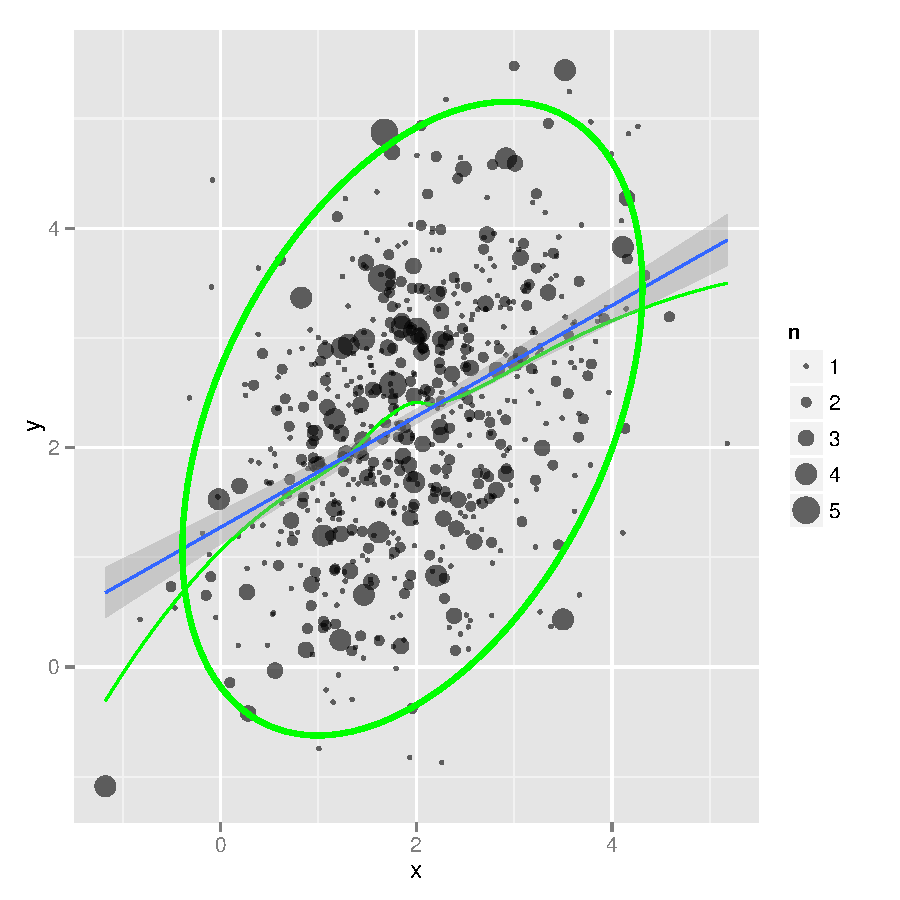
\includegraphics{fig--003}
\caption{Here goes the caption.}
\label{fig:p1}
\end{figure}

\end{document}
